\documentclass[11pt]{article}

\usepackage{latexsym}
\usepackage{amssymb}
\usepackage{amsthm}
\usepackage{graphicx}
\usepackage{enumerate}
\usepackage{amsmath}
\usepackage{cancel}
\numberwithin{equation}{section}

\setlength{\evensidemargin}{.25in}
\setlength{\oddsidemargin}{-.25in}
\setlength{\topmargin}{-.75in}
\setlength{\textwidth}{6.5in}
\setlength{\textheight}{9.5in}
\newcommand{\due}{October 28th, 2015}
\newcommand{\HWnum}{7}
\newcommand{\grad}{\bold\nabla}
\newcommand{\vecE}{\vec{E}}
\newcommand{\scrptR}{\vec{\mathfrak{R}}}
\newcommand{\kapa}{\frac{1}{4\pi\epsilon_0}}
\newcommand{\emf}{\mathcal{E}}
\newcommand{\unit}[1]{\ensuremath{\, \mathrm{#1}}}
\newcommand{\real}{\textnormal{Re}}
\newcommand{\Erf}{\textnormal{Erf}}
\newcommand{\sech}{\textnormal{sech}}
\newcommand{\scrO}{\mathcal{O}}
\newcommand{\levi}{\widetilde{\epsilon}}
\newcommand{\partiald}[2]{\ensuremath{\frac{\partial{#1}}{\partial{#2}}}}
\newcommand{\norm}[2]{\langle{#1}|{#2}\rangle}
\newcommand{\inprod}[2]{\langle{#1}|{#2}\rangle}
\newcommand{\ket}[1]{|{#1}\rangle}
\newcommand{\bra}[1]{\langle{#1}|}





\begin{document}
\begin{titlepage}
\setlength{\topmargin}{1.5in}
\begin{center}
\Huge{Physics 3320} \\
\LARGE{Principles of Electricity and Magnetism II} \\
\Large{Professor Ana Maria Rey} \\[1cm]

\huge{Homework \#\HWnum}\\[0.5cm]

\large{Joe Becker} \\
\large{SID: 810-07-1484} \\
\large{\due} 

\end{center}

\end{titlepage}



\section{Problem \#1}
For a rotating frame we have \emph{Euler's Equation} given by
\begin{equation}
\frac{d\mathbf{L}}{dt} + \pmb{\omega}\times\mathbf{L} = \pmb{\Gamma}^{ext}
\label{Euler}
\end{equation}
Which for torque-free motion we have $\pmb{\Gamma}^{ext} = 0$. Given that the angular
momentum is given by
$$\mathbf{L} = \overleftrightarrow{\mathbf{I}}\cdot\pmb{\omega}$$
where $\overleftrightarrow{\mathbf{I}}$ is the moment of inertia tensor. For an asymmetric 
top we have $I_1<I_2<I_3$ which for torque-free motion gives us three components to equation
\ref{Euler} as
\begin{align*}
I_1\dot{\omega}_1 &= \omega_{2}\omega_{3}(I_2-I_3)\\
I_2\dot{\omega}_2 &= \omega_{3}\omega_{1}(I_3-I_1)\\
I_3\dot{\omega}_3 &= \omega_{1}\omega_{2}(I_1-I_2)
\end{align*}
Given the constraint on the motion $2EI_2 = L^2$ and the constants of motion
\begin{align*}
E &= \frac{1}{2}\left(I_1\omega_1^2+I_2\omega_2^2+I_3\omega_3^2\right)\\
L^2 &= I_1^2\omega_1^2+I_2^2\omega_2^2+I_3^2\omega_3^2
\end{align*}
We can solve for $\omega_1$ in terms of $\omega_2$ by
\begin{align*}
2EI_2 &= L^2\\
\Downarrow\\
I_1I_2\omega_1^2+I_2^2\omega_2^2+I_2I_3\omega_3^2 &= I_1^2\omega_1^2+I_2^2\omega_2^2+I_3^2\omega_3^2\\
\omega_1^2(I_1I_2-I_1^2) &= \omega_3^2(I_3^2-I_2I_3)\\
\omega_1^2 &= \frac{I_3^2-I_2I_3}{I_1I_2-I_1^2}\omega_3^2
\end{align*}
Using this relation we can get a relation between $\omega_1$ and $\omega_2$ by
\begin{align*}
L^2 &= I_1^2\omega_1^2+I_2^2\omega_2^2+I_3^2\omega_3^2\\
&\Downarrow\\
L^2-I_2^2\omega_2^2 &= \left(I_1^2+\frac{I_1I_2-I_1^2}{I_3^2-I_2I_3}I_3^2\right)\omega_1^2\\
&\Downarrow\\
\omega_1^{2} &= \left(L^2-I_2^2\omega_2^2\right)\left(I_1^2+\frac{(I_1I_2-I_1^2)I_3}{I_3-I_2}\right)^{-1}\\
&= \left(L^2-I_2^2\omega_2^2\right)\left(\frac{I_1^2I_3-I_1^2I_2+(I_1I_2-I_1^2)I_3}{I_3-I_2}\right)^{-1}\\
&= \left(L^2-I_2^2\omega_2^2\right)\left(\frac{I_1I_2I_3-I_1^2I_2}{I_3-I_2}\right)^{-1}\\
&= \left(L^2-I_2^2\omega_2^2\right)\left(\frac{I_1I_2(I_3-I_1)}{I_3-I_2}\right)^{-1}\\
&= \left(L^2-I_2^2\omega_2^2\right)\frac{I_3-I_2}{I_1I_2(I_3-I_1)}\\
&= \left(2E-I_2\omega_2^2\right)\frac{I_3-I_2}{I_1(I_3-I_1)}
\end{align*}
Next we can use $E$ to find a relation between $\omega_3$ and $\omega_2$ by
\begin{align*}
2E &= I_1\omega_1^2+I_2\omega_2^2+I_3\omega_3^2\\
&\Downarrow\\
2E - I_2\omega_2^2 &= \left(I_3+I_1\frac{I_3^2-I_2I_3}{I_1I_2-I_1^2}\right)\omega_3^2\\
2E - I_2\omega_2^2 &= \left(I_3+\frac{I_3^2-I_2I_3}{I_2-I_1}\right)\omega_3^2\\
2E - I_2\omega_2^2 &= \left(\frac{I_2I_3-I_1I_3+I_3^2-I_2I_3}{I_2-I_1}\right)\omega_3^2\\
2E - I_2\omega_2^2 &= \left(\frac{I_3(I_3-I_1)}{I_2-I_1}\right)\omega_3^2\\
&\Downarrow\\
\omega_3^2 &= (2E - I_2\omega_2^2)\frac{I_2-I_1}{I_3(I_3-I_1)}
\end{align*}
So now we can solve the integral for $\omega_2$ 
\begin{align*}
I_2\dot{\omega}_2 &= \omega_{3}\omega_{1}(I_3-I_1)\\
&\Downarrow\\
\dot{\omega}_2 &= \frac{I_3-I_1}{I_2}\left((2E - I_2\omega_2^2)^2\frac{I_3-I_2}{I_1(I_3-I_1)}\frac{I_2-I_1}{I_3(I_3-I_1)}\right)^{1/2}\\
&= \frac{2E-I_2\omega_2^2}{I_2}\left(\frac{(I_3-I_2)(I_2-I_1)}{I_1I_3}\right)^{1/2}\\
&= \left(\frac{(2E)^2}{L^2}-\omega_2^2\right)\left(\frac{(I_3-I_2)(I_2-I_1)}{I_1I_3}\right)^{1/2}\\
\frac{d\omega_2}{dt} &= (\omega_{\infty}^2-\omega_2^2)\left(\frac{(I_3-I_2)(I_2-I_1)}{I_1I_3}\right)^{1/2}\\
&\Downarrow\\
\int\frac{d\omega_2}{(1-(\omega_2/\omega_{\infty})^2)} &= \int\omega_{\infty}^2\left(\frac{(I_3-I_2)(I_2-I_1)}{I_1I_3}\right)^{1/2}dt\\
\omega_{\infty}\tanh^{-1}\left(\omega_2/\omega_{\infty}\right) &= \omega_{\infty}\frac{t}{\tau}\\
&\Downarrow\\
\omega_2(t) &= \omega_{\infty}\tanh(t/\tau)
\end{align*}
Note  we defined two new variables by
\begin{align*}
\omega_{\infty} &\equiv \frac{2E}{L}\\
\tau^{-1} &\equiv \omega_{\infty}\left(\frac{(I_3-I_2)(I_2-I_1)}{I_1I_3}\right)^{1/2}
\end{align*}
Now we can use the solution for $\omega_2(t)$ to find the solution for $\omega_1$ by noting 
that
$$\dot{\omega}_2 = \omega_{\infty}\tau^{-1}\sech^2(t/\tau)$$
So we can solve for $\omega_1$ by
\begin{align*}
I_2\dot{\omega}_2 &= \omega_{3}\omega_{1}(I_3-I_1)\\
&\Downarrow\\
I_2\omega_{\infty}\tau^{-1}\sech^2(t/\tau)&= \left(\frac{I_1(I_2-I_1)}{I_3(I_3-I_2)}\right)^{1/2}\omega_{1}^2(I_3-I_1)\\
&\Downarrow\\
\omega_{1}^2 &= \omega_{\infty}^2\sech^2(t/\tau)\frac{I_2(I_3-I_2)}{I_1(I_3-I_1)}\\
\omega_{1}(t) &= \omega_{\infty}\left(\frac{I_2(I_3-I_2)}{I_1(I_3-I_1)}\right)^{1/2}\sech(t/\tau)
\end{align*}
And we can find $\omega_3$ from $\omega_1$ by
\begin{align*}
\omega_3 &= \left(\frac{I_1I_2-I_1^2}{I_3^2-I_2I_3}\right)^{1/2}\omega_1(t)\\
&= \omega_{\infty}\left(\frac{I_2(I_3-I_2)}{I_1(I_3-I_1)}\right)^{1/2}\left(\frac{I_1I_2-I_1^2}{I_3^2-I_2I_3}\right)^{1/2}\sech(t/\tau)\\
&= \omega_{\infty}\left(\frac{I_2(I_2-I_1)}{I_3(I_3-I_1)}\right)^{1/2}\sech(t/\tau)
\end{align*}
So the solutions are
\begin{align*}
\omega_{1}(t) &= \omega_{\infty}\left(\frac{I_2(I_3-I_2)}{I_1(I_3-I_1)}\right)^{1/2}\sech(t/\tau)\\
\omega_2(t) &= \omega_{\infty}\tanh(t/\tau)\\
\omega_3(t) &= \omega_{\infty}\left(\frac{I_2(I_2-I_1)}{I_3(I_3-I_1)}\right)^{1/2}\sech(t/\tau)
\end{align*}
We can use these to write 
$$\omega^2(t) = \omega_{\infty}^2\left(\tanh^2(t/\tau)+\sech^2(t/\tau)\frac{I_2}{I_3-I_1}\left(\frac{I_2-I_1}{I_3}+\frac{I_3-I_2}{I_1}\right)\right)$$
We note that the constrant $I_1<I_2<I_3$ forces the constant multipling the $\sech^2(t/\tau)$ is
$$C\equiv\frac{I_2}{I_3-I_1}\left(\frac{I_2-I_1}{I_3}+\frac{I_3-I_2}{I_1}\right) > 0$$
we see that there are three cases for $\omega^2(t)$ the trivial case when $C=1$ we have 
$\omega^2(t)=\omega_{\infty}^2$ which remains constant in time. The second case where $0<C<1$
we have the case where $\omega^2(t)$ starts at $C$ and grows to $\omega_{\infty}^2$ as $t$ 
increases. The third case is when $C>1$ we have $\omega^2(t)$ again starting at $C$ but 
decreases to $\omega_{\infty}^2$ as $t$ increases. This implies that as $t\rightarrow\infty$
the only axis of rotation becomes $\omega_2$ rotating at a rate of $\omega_{\infty}$.

\pagebreak

\section{Problem \#2}
\begin{enumerate}[(a)]
\item For the torque-free symmetric top we have the potential energy given as
$$V(\theta) = \frac{1}{2I_1}\left(\frac{p_{\phi}-p_{\psi}\cos\theta}{\sin\theta}\right)^2$$
we can find the constant $\theta$ solutions by solving the equation $V'(\theta_0) = 0$. So 
we take a derivative of the potential to get
\begin{align*}
V'(\theta) &= \frac{d}{d\theta}\frac{1}{2I_1}\left(\frac{p_{\phi}-p_{\psi}\cos\theta}{\sin\theta}\right)^2\\
&= \frac{1}{2I_1}2\left(\frac{p_{\phi}-p_{\psi}\cos\theta}{\sin\theta}\right)\frac{p_{\psi}\sin^2\theta-(p_{\phi}-p_{\psi}\cos\theta)\cos\theta}{\sin^2\theta}\\
&= \frac{1}{I_1\sin^3\theta}\left(p_{\phi}-p_{\psi}\cos\theta\right)(p_{\psi}(\sin^2\theta+\cos^2\theta)-p_{\phi}\cos\theta)\\
&= \frac{1}{I_1\sin^3\theta}\left(p_{\phi}-p_{\psi}\cos\theta\right)(p_{\psi}-p_{\phi}\cos\theta)
\end{align*}
So we can see that there are two solutions for $\theta_0$ given by
\begin{align*}
p_{\phi}-p_{\psi}\cos\theta_0 &= 0\\
p_{\psi}-p_{\phi}\cos\theta_0 &= 0
\end{align*}

\item These solutions have corresponding potential energies. For $p_{\phi}=p_{\psi}\cos\theta_0$ we have
$$V(\theta) = \frac{1}{2I_1}\left(\frac{p_{\phi}-p_{\psi}\cos\theta}{\sin\theta}\right)^2 = 0$$
Which corresponds to free rotation with no perturbation. Then for the second solution $p_{\psi}=p_{\phi}\cos\theta_0$ we have
\begin{align*}
V(\theta) &= \frac{1}{2I_1}\left(\frac{p_{\phi}-p_{\psi}\cos\theta}{\sin\theta}\right)^2\\
&= \frac{1}{2I_1}\left(\frac{p_{\phi}-p_{\phi}\cos^2\theta}{\sin\theta}\right)^2\\
&= \frac{1}{2I_1}\left(\frac{p_{\phi}(1-\cos^2\theta)}{\sin\theta}\right)^2\\
&= \frac{1}{2I_1}\left(\frac{p_{\phi}\sin^2\theta}{\sin\theta}\right)^2\\
&= \frac{p_{\phi}^2\sin^2\theta}{2I_1}
\end{align*}
Note that this potential corresponds to the kinetic energy in the angle $\phi$ this would 
correspond to circular movement around the $\hat{e}^{0}_3$ axis. 
\end{enumerate}

\pagebreak

\section{Problem \#3}
\begin{enumerate}[(a)]
\item For a symmetric top in a gravitational potential we have an effective potential given
by
$$V_{eff}(\theta) = \frac{1}{2I_1}\left(\frac{p_{\phi}-p_{\psi}\cos\theta}{\sin\theta}\right)^2 + Mgl\cos\theta$$
Noting the result from problem two we can find the constant $\theta$ solutions by solving
\begin{align*}
V_{eff}'(\theta) = 0 &= \frac{d}{d\theta}\left(\frac{1}{2I_1}\left(\frac{p_{\phi}-p_{\psi}\cos\theta}{\sin\theta}\right)^2 + Mgl\cos\theta\right)\\
&= \frac{1}{I_1\sin^3\theta}\left(p_{\phi}-p_{\psi}\cos\theta\right)(p_{\psi}-p_{\phi}\cos\theta) - Mgl\sin\theta
\end{align*}
We note the equation of motion in the angle $\phi$ given by 
$$\dot{\phi} = \frac{p_{\phi}-p_{\psi}\cos\theta}{I_1\sin^2\theta}$$
This equation is useful because it defines the precession motion as a function of $\theta$. 
Therefore if we find the solutions for $\dot{\phi}$ we can characterize the motion of the top
in a gravitational field. This allows us to replace 
\begin{align*}
V_{eff}'(\theta) = 0 &= \frac{1}{I_1\sin^3\theta}\left(p_{\phi}-p_{\psi}\cos\theta\right)(p_{\psi}-p_{\phi}\cos\theta) - Mgl\sin\theta\\
&\Downarrow\\
0 &= \frac{\dot{\phi}}{\sin\theta}(p_{\psi}-(I_1\sin^2\theta\dot{\phi} + p_{\psi}\cos\theta)\cos\theta) - Mgl\sin\theta\\
0 &= \frac{\dot{\phi}}{\sin\theta}(p_{\psi}(1-\cos^2\theta)-I_1\sin^2\theta\cos\theta\dot{\phi}) - Mgl\sin\theta\\
0 &= \sin\theta\dot{\phi}(p_{\psi}-I_1\theta\cos\theta\dot{\phi}) - Mgl\sin\theta\\
0 &= I_1\cos\theta\dot{\phi}^2 - p_{\psi}\dot{\phi} + Mgl
\end{align*}
So we have a quadratic in $\dot{\phi}$ which we can solve by
$$\dot{\phi} = \frac{p_{\psi}\pm\sqrt{p_{\psi}^2-4I_1\cos\theta{Mgl}}}{2I_1\cos\theta} = \frac{p_{\psi}}{2I_1\cos\theta}\left(1\pm\sqrt{1-\frac{4I_1\cos\theta{Mgl}}{p_{\psi}^2}}\right)$$
We note the condition for real solutions which is given by
$$p_{\psi}^2>4I_1\cos\theta{Mgl}$$
which states that there exists a minimum angular momentum we need to be spinning at so that 
this condition is met. Now we can define a unit-less parameter 
$$x\equiv\frac{2I_1\cos\theta{Mgl}}{p_{\psi}^2}$$
For a small $x$ we can expand to first order in $x$ to find the solutions for $\dot{\phi}$
\begin{align*}
\dot{\phi} &= \frac{p_{\psi}}{2I_1\cos\theta}\left(1\pm\sqrt{1-2x}\right)\\
&= \frac{p_{\psi}}{2I_1\cos\theta}\left(1\pm1-x\right)
\end{align*}
So we have two solutions the first is
\begin{align*}
\dot{\phi} &= \frac{p_{\psi}}{2I_1\cos\theta}\left(x\right)\\
&= \frac{p_{\psi}}{2I_1\cos\theta}\frac{2I_1\cos\theta{Mgl}}{p_{\psi}^2}\\
&= \frac{{Mgl}}{p_{\psi}}
\end{align*}
and
\begin{align*}
\dot{\phi} &= \frac{p_{\psi}}{2I_1\cos\theta}\left(2\right)\\
&= \frac{p_{\psi}}{I_1\cos\theta}
\end{align*}
We note that the first solution $Mgl/p_{\psi}$ corresponds to the zero potential solution 
from problem two and the second solution $p_{\psi}/I_1\cos\theta$ corresponds to the 
constant precession solution.

\item We note the circular solution from the above part 
\begin{align*}
V_{eff}'(\theta) = 0 &= \frac{1}{I_1\sin^3\theta}\left(p_{\phi}-p_{\psi}\cos\theta\right)(p_{\psi}-p_{\phi}\cos\theta) - Mgl\sin\theta\\
&\Downarrow\\
\left(p_{\phi}-p_{\psi}\cos\theta\right) &= \frac{MglI_1\sin^4\theta}{p_{\psi}-p_{\phi}\cos\theta}
\end{align*}
We can use this to evaluate the second derivative of $V_{eff}(\theta)$ by
\begin{align*}
V_{eff}''(\theta) &= \frac{-3\cos\theta}{I_1\sin^4\theta}\left(p_{\phi}-p_{\psi}\cos\theta\right)(p_{\psi}-p_{\phi}\cos\theta) - Mgl\cos\theta + \frac{1}{I_1\sin^3\theta}\frac{d}{d\theta}\left(\left(p_{\phi}-p_{\psi}\cos\theta\right)(p_{\psi}-p_{\phi}\cos\theta)\frac{}{}\right)\\
&= \frac{-3\cos\theta}{I_1\sin^4\theta}MglI_1\sin^4\theta - Mgl\cos\theta + \frac{1}{I_1\sin^3\theta}\frac{d}{d\theta}\left(\left(p_{\phi}-p_{\psi}\cos\theta\right)(p_{\psi}-p_{\phi}\cos\theta)\frac{}{}\right)\\
&= -4Mgl\cos\theta + \frac{1}{I_1\sin^3\theta}\left(\left(p_{\phi}-p_{\psi}\cos\theta\right)p_{\phi}\sin\theta+(p_{\psi}-p_{\phi}\cos\theta)p_{\psi}\sin\theta\frac{}{}\right)\\
&= -4Mgl\cos\theta + \frac{1}{I_1\sin^2\theta}\left(p_{\phi}^2 + p_{\psi}^2 - 2p_{\phi}p_{\psi}\cos\theta\right)\\
&= -4Mgl\cos\theta + \frac{1}{I_1\sin^2\theta}\left(p_{\phi}^2 + p_{\psi}^2(\cos^2\theta+\sin^2\theta) - 2p_{\phi}p_{\psi}\cos\theta\right)\\
&= \frac{p_{\psi}^2}{I_1} - 4Mgl\cos\theta + \frac{1}{I_1\sin^2\theta}\left(p_{\phi}^2 + p_{\psi}^2\cos^2\theta - 2p_{\phi}p_{\psi}\cos\theta\right)\\
&= \frac{p_{\psi}^2}{I_1} - 4Mgl\cos\theta + \frac{(p_{\phi}-p_{\psi}\cos\theta)^2}{I_1\sin^2\theta}
\end{align*}
\end{enumerate}

\pagebreak

\section{Problem \#4}
\begin{enumerate}[(a)]
\item For a symmetric top in a gravitational field with the initial conditions
$$\dot{\phi} = 2\left(\frac{Mgl}{3I_1}\right)^{1/2},\qquad \theta=\frac{\pi}{3},\qquad \dot{\theta}=0,\qquad \dot{\psi}=(3I_1-I_3)\left(\frac{Mgl}{3I_1I_3^2}\right)^{1/2}$$
This system has a Lagrangian that is given by
system as
$$L = \frac{1}{2}I_1(\dot{\theta}^2+\sin^2\theta\dot{\phi}^2) + \frac{1}{2}I_3(\dot{\phi}\cos\theta+\dot{\psi})^2 - Mgl\cos\theta$$
We note the lack of $\phi$ and $\psi$ dependence which implies that there exists conserved 
momenta in $\phi$ and $\psi$ given by
\begin{align*}
p_{\psi} = \partiald{L}{\dot{\psi}} &= I_3(\dot{\phi}\cos\theta+\dot{\psi})\\
p_{\phi} = \partiald{L}{\dot{\phi}} &= I_1\sin^2\theta\dot{\phi} + I_3(\dot{\phi}\cos\theta+\dot{\psi})\cos\theta \\
&= I_1\sin^2\theta\dot{\phi} + p_{\psi}\cos\theta \\
\end{align*}
Using the given initial conditions we can calculate the conserved momenta as
\begin{align*}
p_{\psi} &= I_3(\dot{\phi}\cos\theta+\dot{\psi})\\
&= I_3\left(\left(2\frac{Mgl}{3I_1}\right)^{1/2}\cos(\pi/3)+(3I_1-I_3)\left(\frac{Mgl}{3I_1I_3^2}\right)^{1/2}\right)\\
&= I_3\left(\frac{Mgl}{3I_1}\right)^{1/2}\left(1+(3I_1-I_3)\left(\frac{1}{I_3^2}\right)^{1/2}\right)\\
&= I_3\left(\frac{Mgl}{3I_1}\right)^{1/2}\left(1+3\frac{I_1}{I_3}-\frac{I_3}{I_3}\right)\\
&= 3I_1\left(\frac{Mgl}{3I_1}\right)^{1/2}
\end{align*}
and
\begin{align*}
p_{\phi} &= I_1\sin^2\theta\dot{\phi} + p_{\psi}\cos\theta \\
&= I_1\sin^2(\pi/3)2\left(\frac{Mgl}{3I_1}\right)^{1/2} + 3I_1\left(\frac{Mgl}{3I_1}\right)^{1/2}\cos(\pi/3) \\
&= I_1\left(\frac{Mgl}{3I_1}\right)^{1/2}\left(\frac{3}{2} + \frac{3}{2}\right) \\
&= 3I_1\left(\frac{Mgl}{3I_1}\right)^{1/2}
\end{align*}
We note that the effective potential is given by the $\dot{\phi}^2$ and the $Mgl\cos\theta$
terms as they are the only functions that depend on the non-dotted coordinates. Neglecting 
the constant terms this is given by
\begin{align*}
V_{eff}(\theta) &= \frac{1}{2I_1}\left(\frac{p_{\phi}-p_{\psi}\cos\theta}{\sin\theta}\right)^2 + Mgl\cos\theta\\
&= \frac{1}{2I_1\sin^2\theta}\left(3I_1\left(\frac{Mgl}{3I_1}\right)^{1/2}-3I_1\left(\frac{Mgl}{3I_1}\right)^{1/2}\cos\theta\right)^2 + Mgl\cos\theta\\
&= \frac{9I_1^2}{2I_1\sin^2\theta}\left(\frac{Mgl}{3I_1}\right)\left(1-\cos\theta\right)^2 + Mgl\cos\theta\\
&= \frac{3Mgl}{2\sin^2\theta}\left(1-\cos\theta\right)^2 + Mgl\cos\theta
\end{align*}
\begin{figure}
\centering
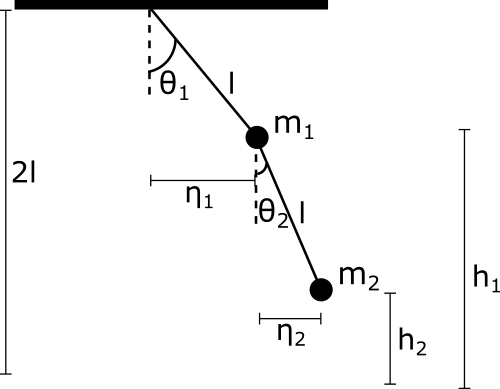
\includegraphics[width=0.8\textwidth]{figure.png}
\caption{Plot of effective potential normalized to $Mgl/I_1$ from $0\le\theta\le{\pi}$.}
\label{figure}
\end{figure}
We plot this potential shown in figure \ref{figure}. We note that this potential implies that
$\theta$ will stabilize around $\theta=0$ as the potential goes to infinity at $\pi$ and $-\pi$.

\item From the above part we know that the total energy is given by
$$E =\frac{1}{2}I_1\dot{\theta}^2 + \frac{3Mgl}{2\sin^2\theta}\left(1-\cos\theta\right)^2 + Mgl\cos\theta$$  
we note that this is a constant which we can solve for by using the given initial conditions
\begin{align*}
E &= \frac{1}{2}I_1\dot{\theta}^2 + \frac{3Mgl}{2\sin^2\theta}\left(1-\cos\theta\right)^2 + Mgl\cos\theta\\
&\Downarrow\\
&= \cancelto{0}{\frac{1}{2}I_1\dot{\theta}^2} + \frac{3Mgl}{2\sin^2(\pi/3)}\left(1-\cos(\pi/3)\right)^2 + Mgl\cos(\pi/3)\\
&= \frac{1}{2}Mgl + \frac{1}{2}Mgl = Mgl
\end{align*}
So we can solve for $\dot{\theta}^2$ as
\begin{align*}
\dot{\theta}^2 &= 2\frac{Mgl}{I_1} - \frac{3Mgl}{I_1\sin^2\theta}\left(1-\cos\theta\right)^2 - 2\frac{Mgl}{I_1}\cos\theta\\
&\Downarrow\\
\sin^2\theta\dot{\theta}^2 &= \frac{Mgl}{I_1}\left(2\sin^2\theta(1-\cos\theta) - 3\left(1-\cos\theta\right)^2\right)\\
\sin^2\theta\dot{\theta}^2 &= \frac{Mgl}{I_1}\left(2(1-\cos^2\theta)(1-\cos\theta) - 3\left(1-\cos\theta\right)^2\right)
\end{align*}
Now we can change variables to $u=\cos\theta$ noting that $\dot{u}^2 = \sin^2\theta\dot{\theta}^2$
this gives us the equation of motion
\begin{align*}
\dot{u}^2 &= \frac{Mgl}{I_1}\left(2(1-u^2)(1-u) - 3\left(1-u\right)^2\right)\\
&= \frac{Mgl}{I_1}\left(2-2u-2u^2+2u^3-3-3u^2+6u\right)\\
&= \frac{Mgl}{I_1}\left(-1+4u-5u^2+2u^3\right)\\
&= \frac{Mgl}{I_1}(1-u)^2(2u-1)
\end{align*}
Next we can solve the differential equation for $u$ by a separation of variables 
\begin{align*}
\frac{du}{(1-u)(2u-1)^{1/2}} &= \left(\frac{Mgl}{I_1}\right)^{1/2}dt\\
&\Downarrow\\
2\tanh^{-1}(\sqrt{2u-1}) &= \left(\frac{Mgl}{I_1}\right)^{1/2}t\\
&\Downarrow\\
2u-1 &= \tanh^2\left(\frac{1}{2}\left(\frac{Mgl}{I_1}\right)^{1/2}t\right)\\
u &= \frac{1}{2}\left(\frac{\cosh(Mgl/I_1t)-1}{\cosh(Mgl/I_1t)+1}+1\right)\\
u &= \frac{\cosh(Mgl/I_1t)}{\cosh(Mgl/I_1t)+1}\\
&\Downarrow\\
\sec\theta &= 1 + \frac{1}{\cosh(Mgl/I_1t)}\\
\sec\theta &= 1 + \sech\left(\frac{Mgl}{I_1}t\right)
\end{align*}
We see that for large $t$ this solution settles at $\theta=0$ which agrees with the qualitative
result in part (a).
\end{enumerate}

\end{document}

